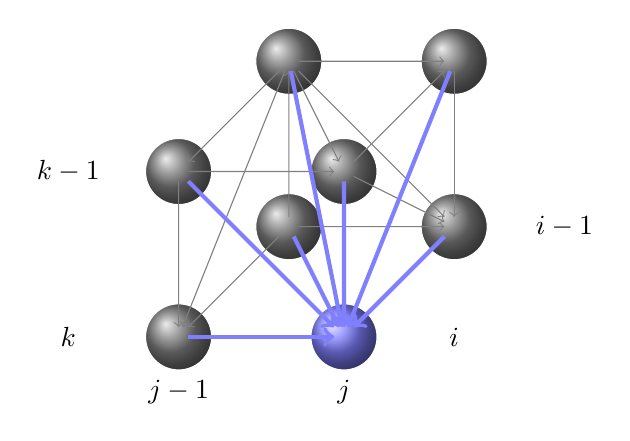
\begin{tikzpicture}[scale=1.4]
\tikzstyle{strnode}=[ball color=gray,white];
\tikzstyle{move}=[line width=1.5pt, blue!50, ->];
\tikzstyle{nomoce} = [gray, ->]
\draw[strnode] (-1.5,1.5) node (v1) {} circle (0.3cm);
\draw[strnode] (-1.5,3) node (v5) {} circle (0.3cm);
\draw[strnode] (0,3) node (v7) {} circle (0.3cm);
\draw[strnode] (0,1.5) node (v4) {} circle (0.3cm);
\draw[strnode, ball color=blue!50] (-1,0.5) node (v2) {} circle (0.3cm);
\draw[strnode] (-2.5,0.5) node (v3) {} circle (0.3cm);
\draw[strnode] (-2.5,2) node (v8) {} circle (0.3cm);
\draw[strnode] (-1,2) node (v6) {} circle (0.3cm);
\draw [nomoce] (v5) edge (v7);
\draw [nomoce] (v7) edge (v4);
\draw [nomoce] (v5) edge (v8);
\draw [nomoce] (v8) edge (v6);
\draw [nomoce] (v6) edge (v7);
\draw [nomoce] (v8) edge (v3);
\draw [nomoce] (v6) edge (v4);
\draw [nomoce] (v5) edge (v6);
\draw [nomoce] (v1) edge (v3);
\draw [nomoce] (v1) edge (v4);
\draw [nomoce] (v1) edge (v5);
\draw [nomoce] (v5) edge (v4);
\draw [nomoce] (v5) edge (v3);
\draw [move] (v1) edge (v2);
\draw [move] (v3) edge (v2);
\draw [move] (v4) edge (v2);
\draw [move] (v5) edge (v2);
\draw [move] (v6) edge (v2);
\draw [move] (v7) edge (v2);
\draw [move] (v8) edge (v2);
\node at (1,1.5) {$i-1$};
\node at (0,0.5) {$i$};
\node at (-1,0) {$j$};
\node at (-2.5,0) {$j-1$};
\node at (-3.5,0.5) {$k$};
\node at (-3.5,2) {$k-1$};
\end{tikzpicture}